\documentclass{standalone}
\usepackage{tikz}
\usetikzlibrary{arrows.meta, positioning, calc}

\begin{document}
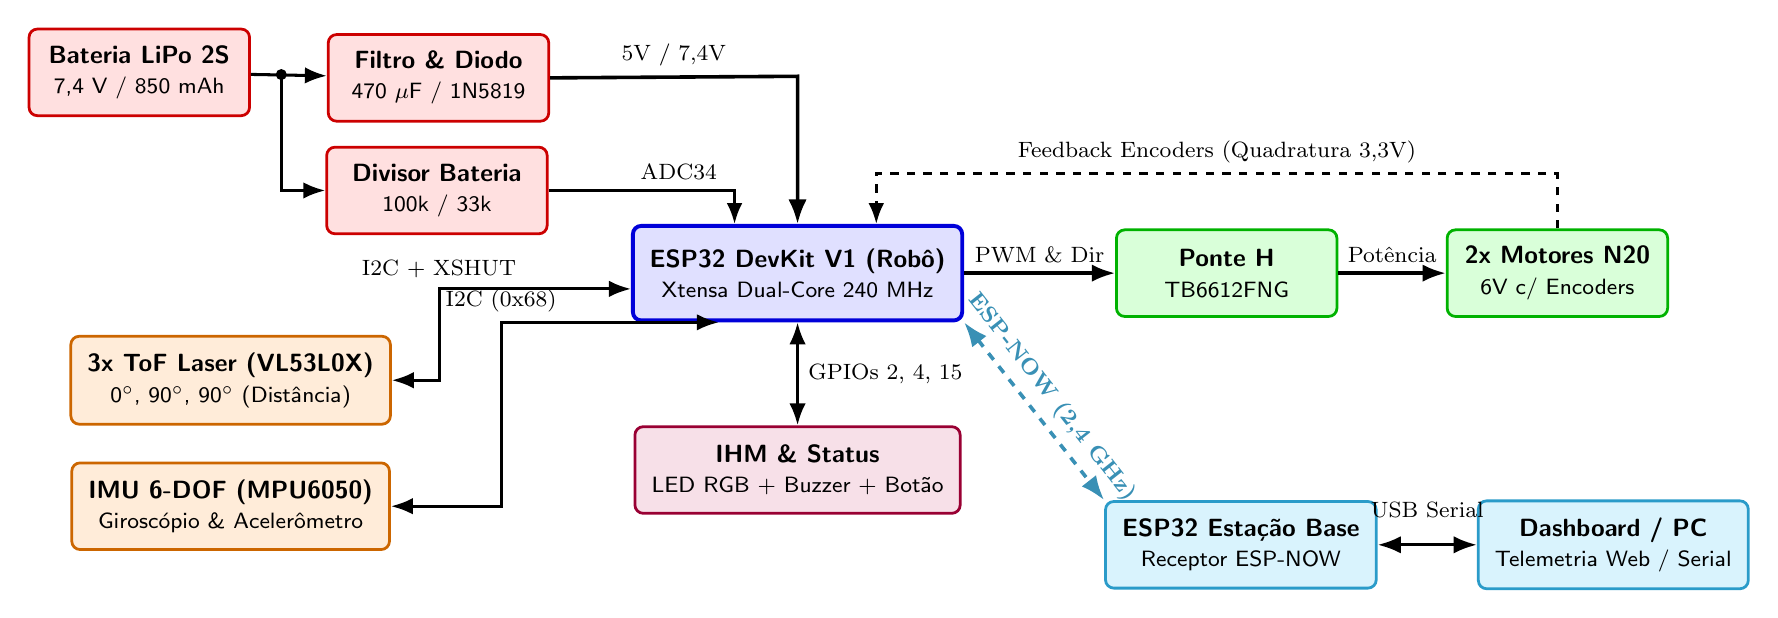
\begin{tikzpicture}[
    font=\sffamily\small,
    >=Latex,
    % Estilos com cores 100% universais (sem risco de tela preta):
    block/.style={rectangle, draw=black!75, line width=1pt, rounded corners=3pt, align=center, inner sep=6pt},
    mcu/.style={block, fill=blue!12, draw=blue!85!black, line width=1.4pt, minimum width=3.4cm, minimum height=1.2cm},
    pwr/.style={block, fill=red!12, draw=red!80!black, minimum width=2.8cm, minimum height=1.1cm},
    sens/.style={block, fill=orange!15, draw=orange!80!black, minimum width=3.0cm, minimum height=1.1cm},
    act/.style={block, fill=green!15, draw=green!70!black, minimum width=2.8cm, minimum height=1.1cm},
    ihm/.style={block, fill=purple!12, draw=purple!80!black, minimum width=3.0cm, minimum height=1.1cm},
    comm/.style={block, fill=cyan!15, draw=cyan!80!black, minimum width=2.8cm, minimum height=1.1cm}
]

    % ================= 1. NÓ CENTRAL (ROBÔ) =================
    \node[mcu] (esp) at (0,0) {\textbf{ESP32 DevKit V1 (Robô)}\\\footnotesize Xtensa Dual-Core 240 MHz};

    % ================= 2. ENERGIA (SUPERIOR ESQUERDO) =================
    \node[pwr] (filtro) at (-4.56, 2.48) {\textbf{Filtro \& Diodo}\\\footnotesize 470 $\mu$F / 1N5819};
    \node[pwr] (batt) at (-8.36, 2.55) {\textbf{Bateria LiPo 2S}\\\footnotesize 7,4 V / 850 mAh};
    \node[pwr] (div) at (-4.58, 1.05) {\textbf{Divisor Bateria}\\\footnotesize 100k / 33k};

    % ================= 3. SENSORES (INFERIOR ESQUERDO - CORES CORRIGIDAS) =================
    \node[sens] (tof) at (-7.2, -1.36) {\textbf{3x ToF Laser (VL53L0X)}\\\footnotesize 0$^\circ$, 90$^\circ$, 90$^\circ$ (Distância)};
    \node[sens] (imu) at (-7.2, -2.96) {\textbf{IMU 6-DOF (MPU6050)}\\\footnotesize Giroscópio \& Acelerômetro};

    % ================= 4. ATUAÇÃO (DIREITA) =================
    \node[act] (drv) at (5.45, 0) {\textbf{Ponte H}\\\footnotesize TB6612FNG};
    \node[act] (mot) at (9.65, 0) {\textbf{2x Motores N20}\\\footnotesize 6V c/ Encoders};

    % ================= 5. IHM (ABAIXO DA ESP32) =================
    \node[ihm] (ihm) at (0, -2.5) {\textbf{IHM \& Status}\\\footnotesize LED RGB + Buzzer + Botão};

    % ================= 6. TELEMETRIA ESP-NOW (INFERIOR DIREITO) =================
    \node[comm] (base) at (5.63, -3.45) {\textbf{ESP32 Estação Base}\\\footnotesize Receptor ESP-NOW};
    \node[comm] (pc) at (10.36, -3.45) {\textbf{Dashboard / PC}\\\footnotesize Telemetria Web / Serial};

    % ================= LIGAÇÕES ELETROELETRÔNICAS LIMPAS =================

    % Linhas de Alimentação
    \draw[->, line width=1.1pt] (batt) -- (filtro);
    \draw[->, line width=1.1pt] ($(batt.east)!0.4!(filtro.west)$) |- (div.west);
    \fill ($(batt.east)!0.4!(filtro.west)$) circle (2pt);
    \draw[->, line width=1.3pt] (filtro.east) -- node[above, font=\footnotesize] {5V / 7,4V} (0, 2.5) -- (esp.north);
    \draw[->, line width=1.0pt] (div.east) -| node[pos=0.35, above, font=\footnotesize] {ADC34} ([xshift=-8mm]esp.north);

    % Linhas de Sensores (Sem cruzar a IHM)
    \draw[<->, line width=1.1pt] (tof.east) -- ++(0.6, 0) |- node[above, font=\footnotesize] {I2C + XSHUT} ([yshift=-2mm]esp.west);
    \draw[<->, line width=1.1pt] (imu.east) -- ++(1.4, 0) |- node[font=\footnotesize, above] {I2C (0x68)} ([xshift=-10mm]esp.south);

    % Linha de IHM (Vertical direta)
    \draw[<->, line width=1.1pt] (esp.south) -- node[right, font=\footnotesize] {GPIOs 2, 4, 15} (ihm.north);

    % Linhas de Motores
    \draw[->, line width=1.2pt] (esp.east) -- node[above, font=\footnotesize] {PWM \& Dir} (drv.west);
    \draw[->, line width=1.2pt] (drv.east) -- node[above, font=\footnotesize] {Potência} (mot.west);

    % Feedback de Encoders (Retorno limpo por cima da Ponte H)
    \draw[->, dashed, line width=1pt] (mot.north) -- ++(0, 0.7) -| node[pos=0.25, above, font=\footnotesize] {Feedback Encoders (Quadratura 3,3V)} ([xshift=10mm]esp.north);

    % Enlace Sem Fio ESP-NOW (Diagonal tracejada ciano)
    \draw[<->, dashed, line width=1.3pt, cyan!70!black] (esp.south east) -- node[above, sloped, font=\footnotesize] {\textbf{ESP-NOW (2,4 GHz)}} (base.north west);

    % Estação Base -> PC (Serial USB)
    \draw[<->, line width=1.2pt] (base.east) -- node[above=6pt, font=\footnotesize] {USB Serial} (pc.west);

\end{tikzpicture}
\end{document}
